% !Mode:: "TeX:UTF-8"
%!TEX program  = xelatex

\documentclass[bwprint]{cumcmthesis} 
%\usepackage{CJK*}
\usepackage{lscape}
\usepackage{cite}
\usepackage{listings}
%\usepackage{xcolor}
%\lstset{
%	numbers=left, 
%	numberstyle= \tiny, 
%	keywordstyle= \color{ blue!70},
%	commentstyle= \color{red!50!green!50!blue!50}, 
%	frame=shadowbox, % 阴影效果
%	rulesepcolor= \color{ red!20!green!20!blue!20} ,
%	escapeinside=``, % 英文分号中可写入中文
%	xleftmargin=2em,xrightmargin=2em, aboveskip=1em,
%	framexleftmargin=2em
%} 


\title{新高考改革下选科组合预测及排课模型}
\tihao{A}
\baominghao{4321}
\schoolname{XX大学}
\membera{小米}
\memberb{向左}
\memberc{哈哈}
\supervisor{老师}
\yearinput{2015}
\monthinput{08}
\dayinput{22}
\begin{document}
 \maketitle
 \begin{abstract}
% 国务院发布的《国务院关于深化考试招生制度改革的实施意见》提出,启动高考综合改革试点,高考成绩由文理分科变成了语数英+3的考试模式,多元评价多元录取。然而新高考改革为人才选拔提供便利的同时,共20种不同的选科组合也为学校的排课及师资分配、教学设施分配提出了挑战,如何预测选择各个组合的学生人数,在不冲突的情况下高效利用资源,将成为本文的研究重点。
 
 随着高考制度的深化改革,“走班制”教学模式逐渐替代传统的高中教学方式.这种教学模式的启用,导致影响排课效率的因素和约束条件增多,并且会出现教学资源匮乏的情况。传统的人工编排课表的方式需要花费工作人员大量的时间,且排出的课表不宜调整,已经无法满足“走班制”教学体制的排课需求。根据对现有排课算法存在的问题的分析,结合“走班制”高中教学的特殊性,建立了相应的数学模型、分析了“走班制”教学模式下排课算法需要设计的约束条件。


针对问题一,我们确立了影响学生选科的三个主要因素,对高中教学质量、大学专业录取和学生的心理及性别等影响因素进行了综合全面的考察。通过搜集数据和计算分析数据得到了回归模型的三组变量:学校教学水平指导值、专业选择指导值和性别指导值。然后使用MEP多表达式编程算法训练得到了各影响因子之间的关系。最后通过数据拟合对模型进行了修正。测得最终误差值为7.75\%。

针对问题二及问题三,分别对改革前和改革后的各种资源差距进行分析。搜集教师工资、教室规模等现有资源的分配数据并进行量化和标准化处理,再依据问题一预测出的各组合学生数量推断教室和教师需求量,进一步推断出改革实行当年的资金缺口。


针对问题四,借助问题一中提出的“绑定值”,并结合各科选科人数,提出了“菜单式”选科组合建议及评价方法。

针对问题五,该问题可归类为多约束优化问题,团队采用遗传算法解决此问题。在解决的过程中,发现遗传算子在染色体交叉过程中存在交叉互斥问题。考虑到排课问题与0-1背包问题在某些程度上拥有较高相似性,因此,在交叉环节,拟采用禁忌搜索算法对其进行约,以保证交叉后的算子仍保持可行状态,减少后续工作量。由于禁忌搜索算法天然的严格性,导致算法在运算过程中,占用大量的资源进行边界条件的判定及变量比较,且如何设置禁忌表、禁忌期限与渴望准则,亦成为难点之一。因此,团队考虑在遗传算法交叉环节中,只保留禁忌搜索算法经典的回溯思想,将其余不重要的因素抛弃;在变异环节,考虑将一周时间内各班级课程随机互换,以达到变异效果。

最终,本文给出一组可行的排课方案,并以课表的样式进行展示,同时对迭代过程中适值函数的变化进行可视化,结果表明本文提出的算法能够在一定程度上提高排课效率,推动高考改革进行。

\keywords{选科组合预测\quad  排课问题\quad   遗传算法\quad  禁忌搜索算法\quad 多表达式编程}
\end{abstract}

\section{问题重述}
\subsection{引言}
新高考改革方向的正确性被大多数教师及教育工作者所认可,改革扩大了学生的学科选择权,考试选择权和课程选择权。\cite{杨德军2017基于新高考的普通高中学生模拟选课调查及分析}然而,更为尖锐的问题也随之产生:部分地区部分学校的师资力量、教学资源可能无法支持新高考改革下的走班制,导致高考改革阻力加大,如何平衡学生选择与学校资源,成为改革路上的第一个难题。
\subsection{问题的提出}
围绕高考改革3+3选科制组合人数、分班情况、排课情况,本文依次提出如下问题:

(1)根据学校的学生规模,文化传统和特色,建立预测模型,估算每一组选科组合的人数。

(2)选科走班制对学校师资力量、教学资源提出了更高的要求,为尽快填补资源缺口,应首先进行合理的缺口分析与计算。

(3)走班制对各种资源,如教师数量、教室数量、教学设备、实验仪器等方面提出了更为严苛的要求,细化每一缺口的成本与解决方案,确定选科组合的边界条件。

(4)“菜单式”选择能够在一定程度上平衡学生选择与学校资源的需求,设立合理的“菜单式”选项,确定最优组合方案。

(5)合理排课对学校提出了更高的要求,在保证教学活动正常进行的情况下,还要尽可能多地考虑教师教学质量与学生学习环境的稳定性,做到“走”与“稳”相结合,让改革的红利切实落在学生身上。


\section{问题分析}
\subsection{问题一分析}
学生选科受到各种因素的影响,因此预测各组合的选科人数也十分复杂,很难在一个模型中全面考虑各个因素的综合影响。为了更好地解决此问题,我们分析了题目及当前各教育领域的专家学者对新高考改革的评价,建立了多因素综合影响模型,确定了三个主要影响因子及其影响系数,并借此预测了下一级高中生的选科情况。
\subsection{问题二三分析}
资源缺口来源于分班后教学资源无法满足师生需求。因此,为计算资源缺口,必须着手计算分班前资源现有量与分班后资源需求量之间的关系,分析刚性需求与柔性需求。有哪些需求必须得到满足,有哪些需求可以妥协,有哪些需求可以不必满足。团队计划从分班前与分班后两个节点分别计算资源与需求的关系,从而得到资源缺口的分析值。
\subsection{问题四分析}
“菜单式”组合方式可以在一定程度上解决选科组合过多,资源要求高,排课复杂度高等问题,但也会导致一部分同学无法选择自己最擅长的科目,只能退而求其次,选择其他选项。因此,为减少学校资源总体需求,同时尽可能多满足学生选课需求,合理设计“菜单式”选项成为当前解决高考改革选课问题的有效途径之一。
\subsection{问题五分析}
排课问题由来已久,其设计到方方面面的冲突,如教室冲突、教师冲突、时间冲突、学生冲突等情况,特别地,当学生人数与班级数量到达一定程度,排课问题复杂性会急剧升高。团队考虑通过编程,借助粒子群优化算法及设置互斥锁解决此问题。


\section{模型假设}
\begin{itemize}
\item 忽略复读生、插班生对选科情况的影响;
\item 忽略选科结束后志愿修改情况对选科的影响;
\item 只考虑公立学校的财政拨款、工资水平;
\item 假设教师教学质量不受走班的影响。
\item 假设选科后所有科目重要程度大致相当,教师平均周课时相等。
\end{itemize}

\section{符号说明}
\begin{longtable}{cc}
	\toprule
	\makebox[0.4\textwidth][c]{符号}	&  \makebox[0.5\textwidth][c]{意义} \\ \hline
	$S$	    & 学校教学水平指导值\\ %(某科标准化成绩)
	$M$	    & 专业选择指导值 \\ %(科目吸引力)
	$g_{sex}$ & 同一性别性别选择科目学生比 \\ 
	$G_{sex}$ & 同一性别选择科目学生数 \\ 
	$A_{sex}$	& 同一性别学生总人数  \\ 
	$p_{sex}$	& 性别选科概率  \\ 
	$G$	    & 性别指导值 \\ 
	$H$	    & 性别因素影响的理论单科选科人数 \\ 
	$C$	    & MEP因变量 \\ 
	$P_{xyz}$	& 选择x、y、z三科组合的概率 \\ 
	$b$		& 绑定值 \\ 
	$t$		& 理论选科比例  \\ 
	$T$		& 最终修正值 \\ 
	$\Omega_1$&分科前教室数量 \\ 
	$\Omega_2$&分科后教室数量 \\
	$N_0$ &学生人数\\
	$N_1$ &理科生人数\\
	$N_2$ &文科生人数\\
	$\varepsilon$ &教室需求差值\\ 
	$Q$		&教学缺口资金\\
	$a$		&单个教室造价\\
	$E$		&教师缺口资金\\
	$e$		&教师年平均工资\\
	$I_i$	&各科缺口教师数量\\
	\bottomrule
\end{longtable}

\section{模型建立与求解}
\subsection{问题一}
影响学生选科的因素众多,包括个人特长、兴趣爱好、学校优势学科、家庭教育、未来职业选择等,团队通过调研翻阅教育行业专家学者点评及文献报道,选出了三种公认对课程选择影响最大的因素:学校教学水平、未来专业选择、性别。

\subsubsection{5.1.1 学校教学水平指导值}
学校教学与学校师资力量、教学方式、历史沿革息息相关,如某些学校格外擅长物理、数学等科目,有些学校则在文科方面有所专长。因此,学校的优势科目,势必会对学生学科产生指导影响,科目优势程度的高低与选科人数呈正相关。

团队收集了山东省曲阜市2017年市一模八所高中的成绩,以及曲阜师范大学附属中学此次参与模拟考试的校均分,通过与八所学校总体均分相比较,得到该校的优势科目及其优势程度。量化方法为:
\begin{equation}
	S_i = {S_{city}-S_{school}}
\end{equation}

其中,$ S_i $为科目$ i $的标准化成绩,计算方法为校均分与八校均分作差。可认为校均分超越八校均分数值越大,则该学科优势越明显。

% Table generated by Excel2LaTeX from sheet '标准成绩'
\begin{table}[htbp]
	\centering
	\caption{八校均分与校均分比较值}
	\begin{tabular}{p{1.5cm}p{1.5cm}p{2.5cm}p{2.5cm}p{2.5cm}}
		\toprule
		学科    & 满分    & 八校均分   & 校均分   & 标准值 \\
		\midrule
		物理    & 110   & 66.2586  & 73.3320  & 7.0734  \\
		化学    & 100   & 69.1366  & 78.7750  & 9.6384  \\
		生物    & 90    & 60.4280  & 72.4288  & 12.0008  \\
		政治    & 100   & 63.8090  & 79.6780  & 14.6240  \\
		历史    & 100   & 65.0540  & 77.5680  & 13.7590  \\
		地理    & 100   & 60.9620  & 73.4879  & 12.5259  \\
		\bottomrule
	\end{tabular}%
	\label{tab:score}%
\end{table}%

该标准值可认为是成绩主导因素,即学校教学水平指导值。

\begin{figure}[!h]
	\centering
	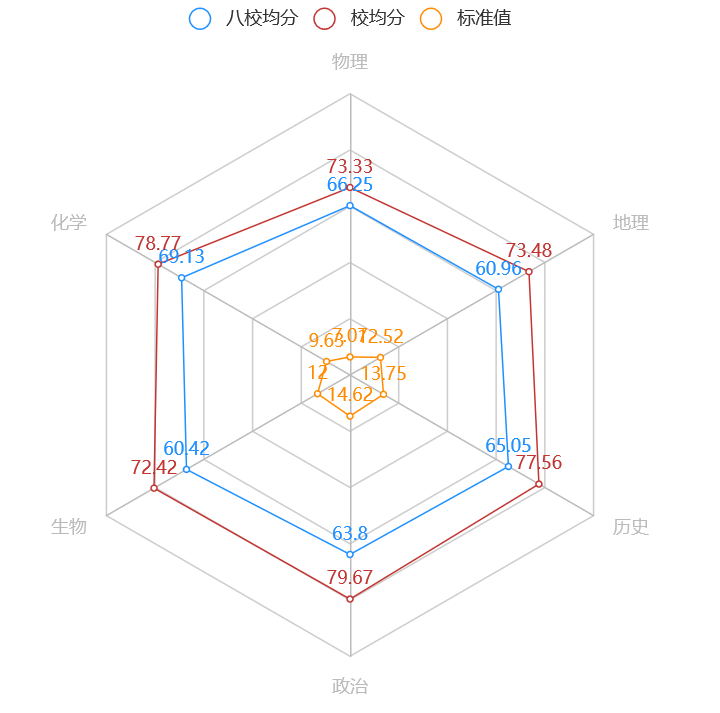
\includegraphics[width=0.5\textwidth]{tab1Rader.png}
	\caption{学校优势学科雷达统计图}
\end{figure}

\subsubsection{5.1.2 专业选择指导值}
未来专业选择亦会对学生选课产生指导作用,如未来就业范围的大小、学科前景、专业未来收入及稳定性。由于未来专业选择命题宽泛,影响因素众多,无法一一列举并量化,因此,团队采用山东省各大学报考分数侧面反映专业火热程度。

团队收集了山东省三所高等综合性学校2017年专业录取成绩,用以量化专业选择因素,具体数据如下表\ref{tab:sdu_per_line}所示。


% Table generated by Excel2LaTeX from sheet 'Sheet1'

	\begin{longtable}{c@{\extracolsep{\fill}}p{2.5cm}cccp{1.8cm}ccc}
		\caption{\label{tab:sdu_per_line}山东大学各学科相关专业及其录取分数线}\\
		\toprule
		& \multicolumn{4}{c}{理工类}       & \multicolumn{4}{c}{文史类} \\
		\midrule
		\multicolumn{1}{l}{学科} &       & 最高分   & 平均分   & 最低分   &       & 最高分   & 平均分   & 最低分 \\
		\midrule
		\multirow{11}[2]{*}{物理} & \textcolor[rgb]{0.333, 0.349, 0.373}{物理学类(泰山学堂、王淦昌班)} & \textcolor[rgb]{0.333, 0.349, 0.373}{650} & \textcolor[rgb]{0.333, 0.349, 0.373}{646} & \textcolor[rgb]{0.333, 0.349, 0.373}{645} &       &       &       &  \\
		& \textcolor[rgb]{0.333, 0.349, 0.373}{物理学类} & \textcolor[rgb]{0.333, 0.349, 0.373}{662} & \textcolor[rgb]{0.333, 0.349, 0.373}{645} & \textcolor[rgb]{0.333, 0.349, 0.373}{639} &       &       &       &  \\
		& \textcolor[rgb]{0.333, 0.349, 0.373}{电气工程及其自动化} & \textcolor[rgb]{0.333, 0.349, 0.373}{651} & \textcolor[rgb]{0.333, 0.349, 0.373}{640} & \textcolor[rgb]{0.333, 0.349, 0.373}{635} & \textcolor[rgb]{0.333, 0.349, 0.373}{} &       &       &  \\
		& \textcolor[rgb]{0.333, 0.349, 0.373}{自动化类} & \textcolor[rgb]{0.333, 0.349, 0.373}{646} & \textcolor[rgb]{0.333, 0.349, 0.373}{634} & \textcolor[rgb]{0.333, 0.349, 0.373}{630} &       &       &       &  \\
		& \textcolor[rgb]{0.333, 0.349, 0.373}{能源动力类} & \textcolor[rgb]{0.333, 0.349, 0.373}{639} & \textcolor[rgb]{0.333, 0.349, 0.373}{628} & \textcolor[rgb]{0.333, 0.349, 0.373}{624} &       &       &       &  \\
		& \textcolor[rgb]{0.333, 0.349, 0.373}{工程力学} & \textcolor[rgb]{0.333, 0.349, 0.373}{635} & \textcolor[rgb]{0.333, 0.349, 0.373}{629} & \textcolor[rgb]{0.333, 0.349, 0.373}{623} &       &       &       &  \\
		& \textcolor[rgb]{0.333, 0.349, 0.373}{机械类} & \textcolor[rgb]{0.333, 0.349, 0.373}{650} & \textcolor[rgb]{0.333, 0.349, 0.373}{630} & \textcolor[rgb]{0.333, 0.349, 0.373}{623} &       &       &       &  \\
		& \textcolor[rgb]{0.333, 0.349, 0.373}{建筑学(五年制)} & \textcolor[rgb]{0.333, 0.349, 0.373}{634} & \textcolor[rgb]{0.333, 0.349, 0.373}{627} & \textcolor[rgb]{0.333, 0.349, 0.373}{623} &       &       &       &  \\
		& \textcolor[rgb]{0.333, 0.349, 0.373}{土木类} & \textcolor[rgb]{0.333, 0.349, 0.373}{634} & \textcolor[rgb]{0.333, 0.349, 0.373}{626} & \textcolor[rgb]{0.333, 0.349, 0.373}{623} &       &       &       &  \\
		& \textcolor[rgb]{0.333, 0.349, 0.373}{集成电路设计与集成系统} & \textcolor[rgb]{0.333, 0.349, 0.373}{635} & \textcolor[rgb]{0.333, 0.349, 0.373}{627} & \textcolor[rgb]{0.333, 0.349, 0.373}{623} &       &       &       &  \\
		& \textcolor[rgb]{0.333, 0.349, 0.373}{电气工程及其自动化(卓越工程师培养计划)} & \textcolor[rgb]{0.333, 0.349, 0.373}{651} & \textcolor[rgb]{0.333, 0.349, 0.373}{648} & \textcolor[rgb]{0.333, 0.349, 0.373}{645} & \textcolor[rgb]{0.333, 0.349, 0.373}{} &       &       &  \\
		\midrule
		\multirow{4}[2]{*}{化学} & \textcolor[rgb]{0.333, 0.349, 0.373}{化学类} & \textcolor[rgb]{0.333, 0.349, 0.373}{644} & \textcolor[rgb]{0.333, 0.349, 0.373}{632} & \textcolor[rgb]{0.333, 0.349, 0.373}{627} &       &       &       &  \\
		& \textcolor[rgb]{0.333, 0.349, 0.373}{化学工程与工艺} & \textcolor[rgb]{0.333, 0.349, 0.373}{645} & \textcolor[rgb]{0.333, 0.349, 0.373}{627} & \textcolor[rgb]{0.333, 0.349, 0.373}{623} &       &       &       &  \\
		& \textcolor[rgb]{0.333, 0.349, 0.373}{材料类} & \textcolor[rgb]{0.333, 0.349, 0.373}{643} & \textcolor[rgb]{0.333, 0.349, 0.373}{631} & \textcolor[rgb]{0.333, 0.349, 0.373}{623} &       &       &       &  \\
		& \textcolor[rgb]{0.333, 0.349, 0.373}{药学类} & \textcolor[rgb]{0.333, 0.349, 0.373}{641} & \textcolor[rgb]{0.333, 0.349, 0.373}{626} & \textcolor[rgb]{0.333, 0.349, 0.373}{623} &       &       &       &  \\
		\midrule
		\multirow{8}[2]{*}{生物} & \textcolor[rgb]{0.333, 0.349, 0.373}{生物科学类} & \textcolor[rgb]{0.333, 0.349, 0.373}{640} & \textcolor[rgb]{0.333, 0.349, 0.373}{629} & \textcolor[rgb]{0.333, 0.349, 0.373}{623} & \textcolor[rgb]{0.333, 0.349, 0.373}{} &       &       &  \\
		& \textcolor[rgb]{0.333, 0.349, 0.373}{生物医学工程} & \textcolor[rgb]{0.333, 0.349, 0.373}{640} & \textcolor[rgb]{0.333, 0.349, 0.373}{627} & \textcolor[rgb]{0.333, 0.349, 0.373}{623} &       &       &       &  \\
		& \textcolor[rgb]{0.333, 0.349, 0.373}{临床药学(五年制)} & \textcolor[rgb]{0.333, 0.349, 0.373}{635} & \textcolor[rgb]{0.333, 0.349, 0.373}{628} & \textcolor[rgb]{0.333, 0.349, 0.373}{623} &       &       &       &  \\
		& \textcolor[rgb]{0.333, 0.349, 0.373}{临床医学(5+3,卓越医生培养计划)} & \textcolor[rgb]{0.333, 0.349, 0.373}{667} & \textcolor[rgb]{0.333, 0.349, 0.373}{657} & \textcolor[rgb]{0.333, 0.349, 0.373}{652} &       &       &       &  \\
		& \textcolor[rgb]{0.333, 0.349, 0.373}{临床医学(5+3)} & \textcolor[rgb]{0.333, 0.349, 0.373}{662} & \textcolor[rgb]{0.333, 0.349, 0.373}{647} & \textcolor[rgb]{0.333, 0.349, 0.373}{641} & \textcolor[rgb]{0.333, 0.349, 0.373}{} &       &       &  \\
		& \textcolor[rgb]{0.333, 0.349, 0.373}{口腔医学(5+3)} & \textcolor[rgb]{0.333, 0.349, 0.373}{653} & \textcolor[rgb]{0.333, 0.349, 0.373}{643} & \textcolor[rgb]{0.333, 0.349, 0.373}{639} &       &       &       &  \\
		& \textcolor[rgb]{0.333, 0.349, 0.373}{临床医学(5+3,儿科方向)} & \textcolor[rgb]{0.333, 0.349, 0.373}{641} & \textcolor[rgb]{0.333, 0.349, 0.373}{635} & \textcolor[rgb]{0.333, 0.349, 0.373}{632} & \textcolor[rgb]{0.333, 0.349, 0.373}{} &       &       &  \\
		& \textcolor[rgb]{0.333, 0.349, 0.373}{预防医学(五年制)} & \textcolor[rgb]{0.333, 0.349, 0.373}{647} & \textcolor[rgb]{0.333, 0.349, 0.373}{632} & \textcolor[rgb]{0.333, 0.349, 0.373}{626} &       &       &       &  \\
		\midrule
		\multirow{3}[2]{*}{政治} & \textcolor[rgb]{0.333, 0.349, 0.373}{法学类} & \textcolor[rgb]{0.333, 0.349, 0.373}{643} & \textcolor[rgb]{0.333, 0.349, 0.373}{637} & \textcolor[rgb]{0.333, 0.349, 0.373}{633} & \textcolor[rgb]{0.333, 0.349, 0.373}{法学类} & \textcolor[rgb]{0.333, 0.349, 0.373}{621} & \textcolor[rgb]{0.333, 0.349, 0.373}{613} & \textcolor[rgb]{0.333, 0.349, 0.373}{609} \\
		&       &       &       &       & \textcolor[rgb]{0.333, 0.349, 0.373}{哲学类} & \textcolor[rgb]{0.333, 0.349, 0.373}{612} & \textcolor[rgb]{0.333, 0.349, 0.373}{605} & \textcolor[rgb]{0.333, 0.349, 0.373}{601} \\
		&       &       &       &       & \textcolor[rgb]{0.333, 0.349, 0.373}{政治学类} & \textcolor[rgb]{0.333, 0.349, 0.373}{613} & \textcolor[rgb]{0.333, 0.349, 0.373}{605} & \textcolor[rgb]{0.333, 0.349, 0.373}{600} \\
		\midrule
		\multirow{2}[2]{*}{历史} &       &       &       &       & \textcolor[rgb]{0.333, 0.349, 0.373}{历史学类} & \textcolor[rgb]{0.333, 0.349, 0.373}{620} & \textcolor[rgb]{0.333, 0.349, 0.373}{611} & \textcolor[rgb]{0.333, 0.349, 0.373}{606} \\
		&       &       &       &       & \textcolor[rgb]{0.333, 0.349, 0.373}{考古学} & \textcolor[rgb]{0.333, 0.349, 0.373}{605} & \textcolor[rgb]{0.333, 0.349, 0.373}{603} & \textcolor[rgb]{0.333, 0.349, 0.373}{600} \\
		\midrule
		\multirow{2}[2]{*}{地理} & \textcolor[rgb]{0.333, 0.349, 0.373}{环境科学与工程类} & \textcolor[rgb]{0.333, 0.349, 0.373}{638} & \textcolor[rgb]{0.333, 0.349, 0.373}{628} & \textcolor[rgb]{0.333, 0.349, 0.373}{623} &       &       &       &  \\
		& \textcolor[rgb]{0.333, 0.349, 0.373}{水利类} & \textcolor[rgb]{0.333, 0.349, 0.373}{627} & \textcolor[rgb]{0.333, 0.349, 0.373}{625} & \textcolor[rgb]{0.333, 0.349, 0.373}{623} &       &       &       &  \\
		\bottomrule
%	\label{tab:sdu_per_linel}%
\end{longtable}%

运用相同的方式,我们收集到了山东大学、山东师范大学以及济南大学三所山东省综合性高水平大学的各专业录取分数线,侧面反映各学科录取竞争的激烈程度,进而反映出学生对各专业的认可度。该认可度可认为是高中生选课的指导因素之一。

由于三所大学水平存在差距,无法直接运用分数线进行学科认可度的衡量,因此,我们通过将各专业平均分与对应学校录取平均分做差值,计算得出标准化数据用以对比。计算方法如下。
\begin{equation}
M_i = M_s-M_l
\end{equation}

其中,$ M_i $表示科目$ i $的专业指导水平,即科目吸引力;$ M_s $表示科目$ i $专业线均分,$ M_l $表示学校录取线均分;

经过标准化处理后的三所综合性高水平大学,各学科指导水平如下表\ref{tab:standard_major_line}所示。

% Table generated by Excel2LaTeX from sheet 'Sheet3'

	\begin{longtable}{cccp{1.5cm}p{1.5cm}p{1.5cm}p{1.5cm}p{2cm}}
		\caption{\label{tab:standard_major_line}三所大学各学科均值及其标准化均值}\\
		\toprule
		学校    & 学校均分  & 学科    & \multicolumn{2}{c}{学科均分} & \multicolumn{3}{c}{标准化均值} \\
		\midrule
		&       &       & 理     & 文     & 理     & 文     & 综合 \\
		\midrule
		\multirow{6}[1]{*}{山东大学} &       & 物理    & 645.00  &       & 12.00  & -     & 12.00  \\
		&       & 化学    & 629.00  &       & -4.00  & -     & -4.00  \\
		& 理:633 & 生物    & 637.25  &       & 4.25  & -     & 4.25  \\
		& 文:607 & 政治    & 637.00  & 607.67  & 4.00  & 0.67  & 2.33  \\
		&       & 历史    &       & 607.00  & -     & 0.00  & 0.00  \\
		&       & 地理    & 626.50  &       & -6.50  & -     & -6.50  \\
		\midrule
		\multirow{6}[1]{*}{山东师范大学} &       & 物理    & 569.67  &       & -3.33  & -     & -3.33  \\
		&       & 化学    & 573.33  &       & 0.33  & -     & 0.33  \\
		& 理:573 & 生物    & 566.33  &       & -6.67  & -     & -6.67  \\
		& 文:567 & 政治    & 560.00  & 559.20  & -13.00  & -7.80  & -10.40  \\
		&       & 历史    &       & 556.00  & -     & -11.00  & -11.00  \\
		&       & 地理    & 558.67  & 559.33  & -14.33  & -7.67  & -11.00  \\
		\midrule
		\multirow{6}[2]{*}{济南大学} &       & 物理    & 536.20  &       & -0.70  & -     & -0.70  \\
		&       & 化学    & 535.33  &       & -1.57  & -     & -1.57  \\
		& 理:574 & 生物    & 531.50  &       & -5.40  & -     & -5.40  \\
		& 文:564 & 政治    & 536.50  & 547.00  & -0.40  & 4.00  & 1.80  \\
		&       & 历史    &       & 545.00  & -     & 2.00  & 2.00  \\
		&       & 地理    & 529.50  &       & -7.40  & -     & -7.40  \\
		\bottomrule
	\end{longtable}%


其中,科目综合标准化均值为文理标准化的均值处理,若不存在文理兼收科目,则独取一科作为综合标准化均值。

将三所学校各科成绩综合,得到6科专业指导值均值$ M_i $
\begin{equation}
M_i = Ave(m_1,m_2,m_3)
\end{equation}

计算结果如下表\ref{tab:final_major_value}所示。
% Table generated by Excel2LaTeX from sheet 'Sheet3'

	\begin{longtable}{p{2.5cm}p{2.5cm}p{1.5cm}p{2.5cm}p{2.5cm}}
		\caption{\label{tab:final_major_value}各学科专业选择指导值}\\
		\toprule
		学科    & \multicolumn{1}{l}{专业指导值} &       & 学科    & \multicolumn{1}{l}{专业指导值} \\
		\midrule
		物理    & 2.66  &       & 政治    & -2.09  \\
		化学    & -1.74  &       & 历史    & -3.00  \\
		生物    & -2.61  &       & 地理    & -8.30  \\
		\bottomrule
	\end{longtable}%


\subsubsection{5.1.3 性别指导值}
性别对学生选课亦产生较大的影响,如男生更倾向于选择理工类科目,女生更倾向于选择文史类科目。在理工类与文史类倾向较大的选课班级中,男女生人数比例常常会失衡到较为严重的程度。
文献\cite{李金波2014高考学科表现的性别差异分析}通过调查获得数据,男女生对于各科目的性别倾向如下表\ref{tab:sex_influence}所示。

% Table generated by Excel2LaTeX from sheet '单科'
	\begin{longtable}{cccccccc}
		\caption{\label{tab:sex_influence}各单科不同性别选择人数及其占比}\\
		\toprule
		科目    & \multicolumn{1}{c}{男生人数} & \multicolumn{1}{c}{男生占比} & \multicolumn{1}{c}{女生人数} & \multicolumn{1}{c}{女生占比} & 男女选科比 & \multicolumn{1}{c}{男生选科概率} & \multicolumn{1}{c}{女生选科概率} \\
		\midrule
		物理    & 1041  & 11.27\% & 477   & 5.17\% & 2.18  & \multicolumn{1}{c}{68.58\%} & \multicolumn{1}{c}{31.42\%} \\
		化学    & 978   & 10.59\% & 468   & 5.07\% & 2.09  & \multicolumn{1}{c}{67.63\%} & \multicolumn{1}{c}{32.37\%} \\
		生物    & 896   & 9.70\% & 604   & 6.54\% & 1.48  & \multicolumn{1}{c}{59.73\%} & \multicolumn{1}{c}{40.27\%} \\
		政治    & 688   & 7.45\% & 914   & 9.90\% & 0.75  & \multicolumn{1}{c}{42.95\%} & \multicolumn{1}{c}{57.05\%} \\
		历史    & 643   & 6.96\% & 886   & 9.59\% & 0.73  & \multicolumn{1}{c}{42.05\%} & \multicolumn{1}{c}{57.95\%} \\
		地理    & 850   & 9.21\% & 789   & 8.54\% & 1.08  & \multicolumn{1}{c}{51.86\%} & \multicolumn{1}{c}{48.14\%} \\
		\midrule
		总     & 5096  & 55.19\% & 4138  & 44.81\% & 1.23  &       &  \\
		\bottomrule
	\end{longtable}%
	\label{}%
	
\begin{figure}[!ht]
	\centering
	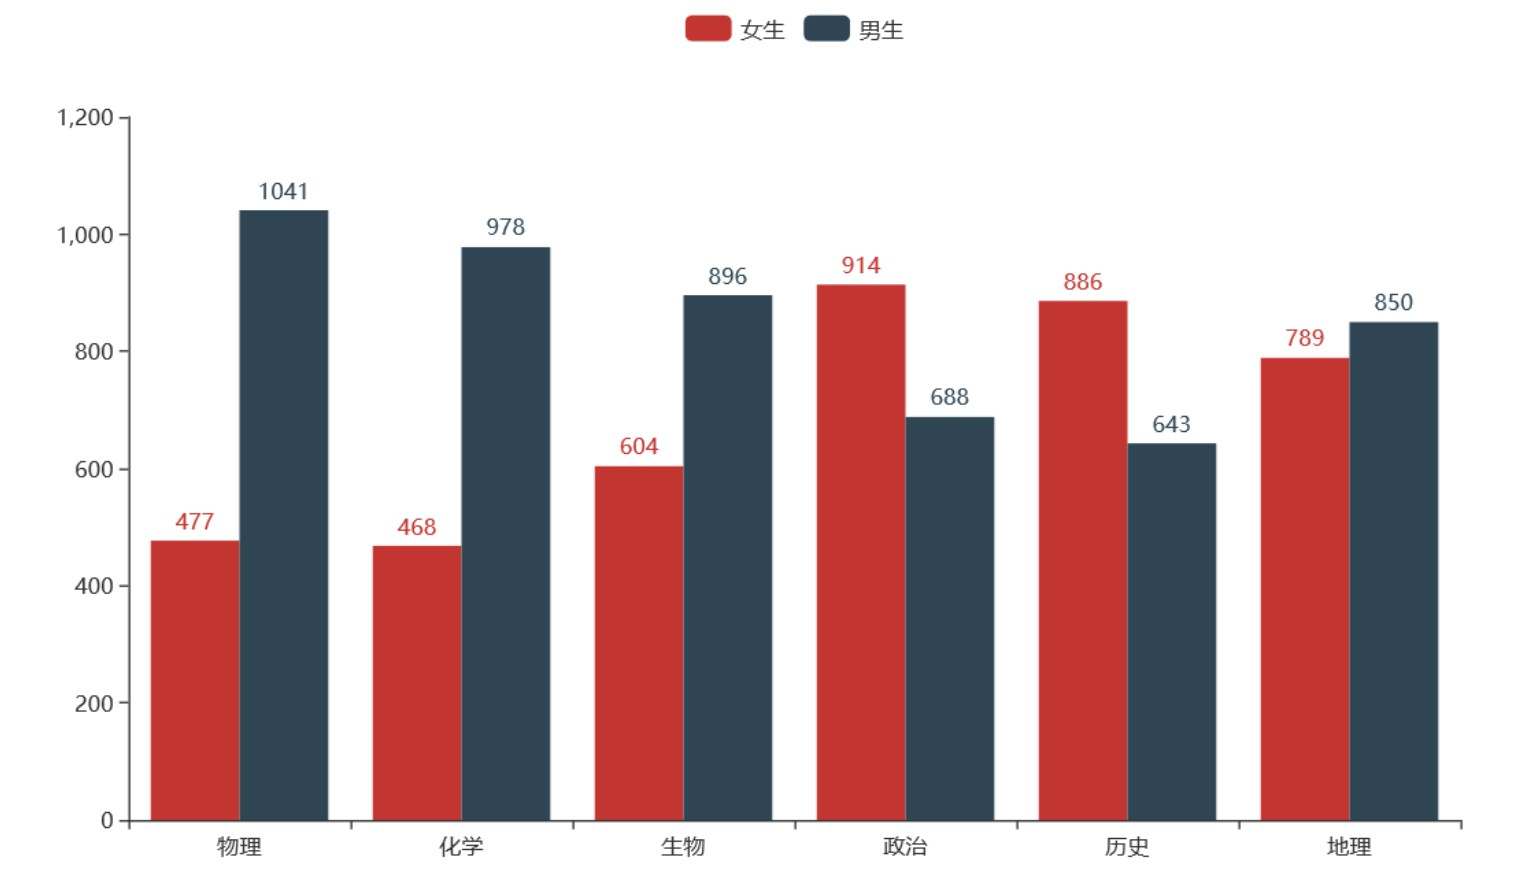
\includegraphics[width=\textwidth]{tab6(3).jpg}
	\caption{单科选科性别差异柱状图}
\end{figure}
	

其中,性别占比为其选科人数在性别总人数中的占比,如物理学科男生占比11.27\%,意味着在1440名男生中,有1041名男生选择物理。性别占比计算公式如下。
\begin{equation}
g = \frac{G_{sex}}{A_{sex}}
\end{equation}
经过此公式的处理后,男女性别占比数据均为标准化数据,即某单科性别选择倾向与总体样本男女比无关。

性别选科概率为标准化后的比值,其计算公式为。

\begin{equation}
P_{male} = \frac{G_{male}}{G_{male}+G_{famale}}
\end{equation}

\begin{equation}
P_{female} = \frac{G_{female}}{G_{male}+G_{famale}}
\end{equation}

以物理为例,若一男生进行选科活动,则该男生出于性别因素,选择物理科目的概率为68.58\%。性别占比经过标准化处理后,使各单科性别倾向与全校性别比无关,此时,通过比较性别占比,即可直观反映出某单科对性别的倾向程度。

性别指导值计算公式如下。

\begin{equation}
\label{gender}
G = \frac{P_{male}*A_{male}+P_{female}*A_{female}}{A_{male}+A_{female}}
\end{equation}

以物理学科为例,团队收集到数据,曲师大附属中学2016级共有3118人,其中男生1440人,女生1678人,通过性别分别加权计算,得到物理性别指导值为0.4909534。

整所学校受性别影响,各单科对男女生吸引力不同,结合学校整体性别比,可求得单一的处于性别因素考虑情况下的单科选科人数。计算公式如下。

\begin{equation}
H = G_{male}*P_{male} + G_{female}*P_{female}
\end{equation}


公式可结合学校整体性别比,计算性别指导下的男女选科人数。

\subsubsection{5.1.4 综合处理}

前期通过对各个因素分析,量化出三项指导值,分别为学校教学水平指导值$ Score $,专业选择指导值$ Major $以及性别指导值$ Gender $。
通过研究发现,三者对最终选课结果的影响程度不同,因此,团队拟采用MEP(Multi Expression Programming)算法,对三者进行函数拟合。为得到训练数据集,前期准备如下:

经调查统计,得到曲阜师范大学附属中学实际选科组合人数,统计数据如下表\ref{tab:school_per_select}所示。该统计数据为学生选课的真实数据,能够真实反映学科组合的受欢迎程度,我们将基于此进行接下来的研究。


% Table generated by Excel2LaTeX from sheet 'Sheet1'
\begin{longtable}{p{2.5cm}p{2.5cm}p{4cm}}
	\caption{\label{tab:school_per_select}各学科单科选科人数统计}\\
	\toprule
	学科    & 选科人数  & 选科人数占比 \\
	\midrule
	物理    & 1573  & 53.27\% \\
	化学    & 1771  & 59.97\% \\
	生物    & 1483  & 50.22\% \\
	政治    & 1099  & 37.22\% \\
	历史    & 1444  & 48.90\% \\
	地理    & 1489  & 50.42\% \\
	\midrule
	总     & 8859  & 300.00\% \\
	\bottomrule
\end{longtable}%

\begin{figure}[!ht]
	\centering
	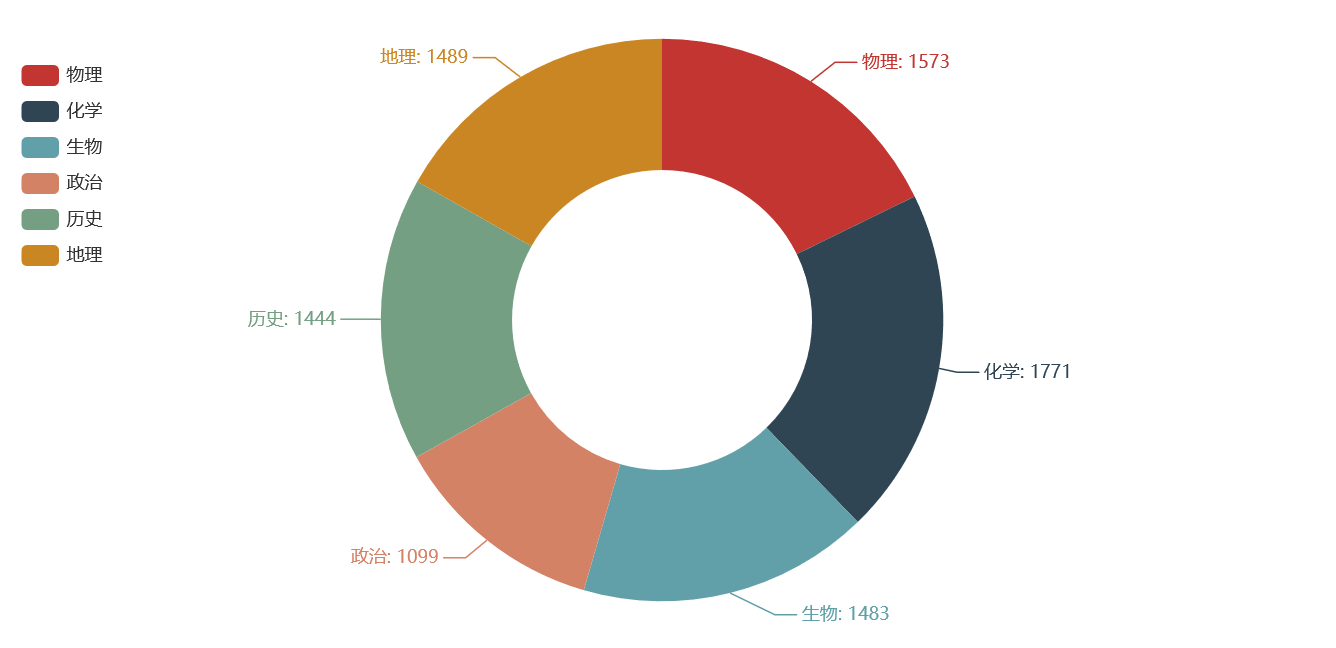
\includegraphics[width=\textwidth]{tab7.png}
	\caption{各单科选科人数占比}
\end{figure}

表格中,选科人数占比未经标准化处理,因学生可任选三门课,故总体选科人数及占比均为标准化数据的三倍。其实际选科人数应为2953人。

经过前期数据收集工作,接下来,可以进行训练集的统计工作,该训练集曲师大附中实际选课情况为依据,具体计算结果如下表\ref{tab:final_result}所示。

% Table generated by Excel2LaTeX from sheet '最终数据'
	\begin{longtable}{p{2cm}p{3cm}p{3cm}p{3cm}p{3cm}}
		\caption{\label{tab:final_result}高中选课数据训练集}\\
		\toprule
		学科    & \multicolumn{1}{l}{Score(subject)} & \multicolumn{1}{l}{Major(subject)} & \multicolumn{1}{l}{Gender(subject)} & \multicolumn{1}{l}{选科比例} \\
		\midrule
		物理    & 7.0733978  & 2.6566700  & 0.4909534  & 0.53  \\
		化学    & 9.6384409  & -1.7445400  & 0.5102595  & 0.60  \\
		生物    & 12.0008030  & -2.6053300  & 0.5074348  & 0.50  \\
		政治    & 14.6240000  & -2.0888800  & 0.5095021  & 0.37  \\
		历史    & 13.7590000  & -3.0000000  & 0.5044439  & 0.49  \\
		地理    & 12.5258560  & -8.2999500  & 0.5016147  & 0.50  \\
		\bottomrule
		
	\end{longtable}%

运用MEP多表达式编程\cite{alavi2010multi}\cite{zhang2012predicting},输入测试数据。
\begin{equation}
C = f(x_0,x_1,x_2)
\end{equation}
其中,$ x_0 $,$ x_1 $,$ x_2 $依次代表$ S $、$ M $、$ G $数值,$ f(x_0,x_2,x_2 $数值为选科比例。
\begin{equation}
C = f(S,M,G)
\end{equation}
基于测试集,算法求解得到函数模型如下。
\begin{equation}
C = |(0.677076+M-ceil(M))*tan(G^2+|log_2(lgS)|)|
\end{equation}
\subsubsection{5.1.5 数值修正}
通过统计发现,选科组合人数理论比例与实际比例差距较大,推测是变量并非相互独立所造成。如表\ref{tab:school_per_select}为各单科选科比值,若学科相互独立,由公式
\begin{equation}
P{xyz} = P_x*P_y*P_z
\end{equation}
可得到所有选科组合理论选科人数比例。下表\ref{tab:20select}为曲师大附中实际选科情况。

% Table generated by Excel2LaTeX from sheet 'Sheet1'

	\begin{longtable}{ccccccc}
		\caption{\label{tab:per_select}分科实际选科数据}\\
		\toprule
		\multicolumn{3}{c}{学科组合} & 选择人数  & 实际选择比例 & 理论选科比例 & 学科组合绑定值 \\
		\midrule
		物理    & 化学    & 生物    & 573   & 19.40\% & 5.35\% & 3.63  \\
		政治    & 历史    & 地理    & 453   & 15.34\% & 3.06\% & 5.02  \\
		地理    & 物理    & 化学    & 238   & 8.06\% & 5.37\% & 1.50  \\
		地理    & 化学    & 生物    & 189   & 6.40\% & 5.06\% & 1.26  \\
		历史    & 物理    & 化学    & 171   & 5.79\% & 5.21\% & 1.11  \\
		历史    & 化学    & 生物    & 148   & 5.01\% & 4.91\% & 1.02  \\
		历史    & 地理    & 生物    & 123   & 4.17\% & 4.13\% & 1.01  \\
		地理    & 物理    & 生物    & 121   & 4.10\% & 4.50\% & 0.91  \\
		历史    & 地理    & 化学    & 119   & 4.03\% & 4.93\% & 0.82  \\
		政治    & 物理    & 化学    & 118   & 4.00\% & 3.96\% & 1.01  \\
		历史    & 地理    & 物理    & 101   & 3.42\% & 4.38\% & 0.78  \\
		政治    & 历史    & 化学    & 98    & 3.32\% & 3.64\% & 0.91  \\
		政治    & 历史    & 生物    & 81    & 2.74\% & 3.05\% & 0.90  \\
		政治    & 历史    & 物理    & 79    & 2.68\% & 3.23\% & 0.83  \\
		政治    & 化学    & 生物    & 76    & 2.57\% & 3.74\% & 0.69  \\
		历史    & 物理    & 生物    & 71    & 2.40\% & 4.36\% & 0.55  \\
		政治    & 地理    & 物理    & 52    & 1.76\% & 3.33\% & 0.53  \\
		政治    & 地理    & 生物    & 52    & 1.76\% & 3.14\% & 0.56  \\
		政治    & 物理    & 生物    & 49    & 1.66\% & 3.32\% & 0.50  \\
		政治    & 地理    & 化学    & 41    & 1.39\% & 3.75\% & 0.37  \\
		\midrule
		\multicolumn{3}{c}{总} & 2953  & 1     &       &  \\
		\bottomrule
		\label{tab:20select}
	\end{longtable}%

\begin{figure}[!ht]
	\centering
	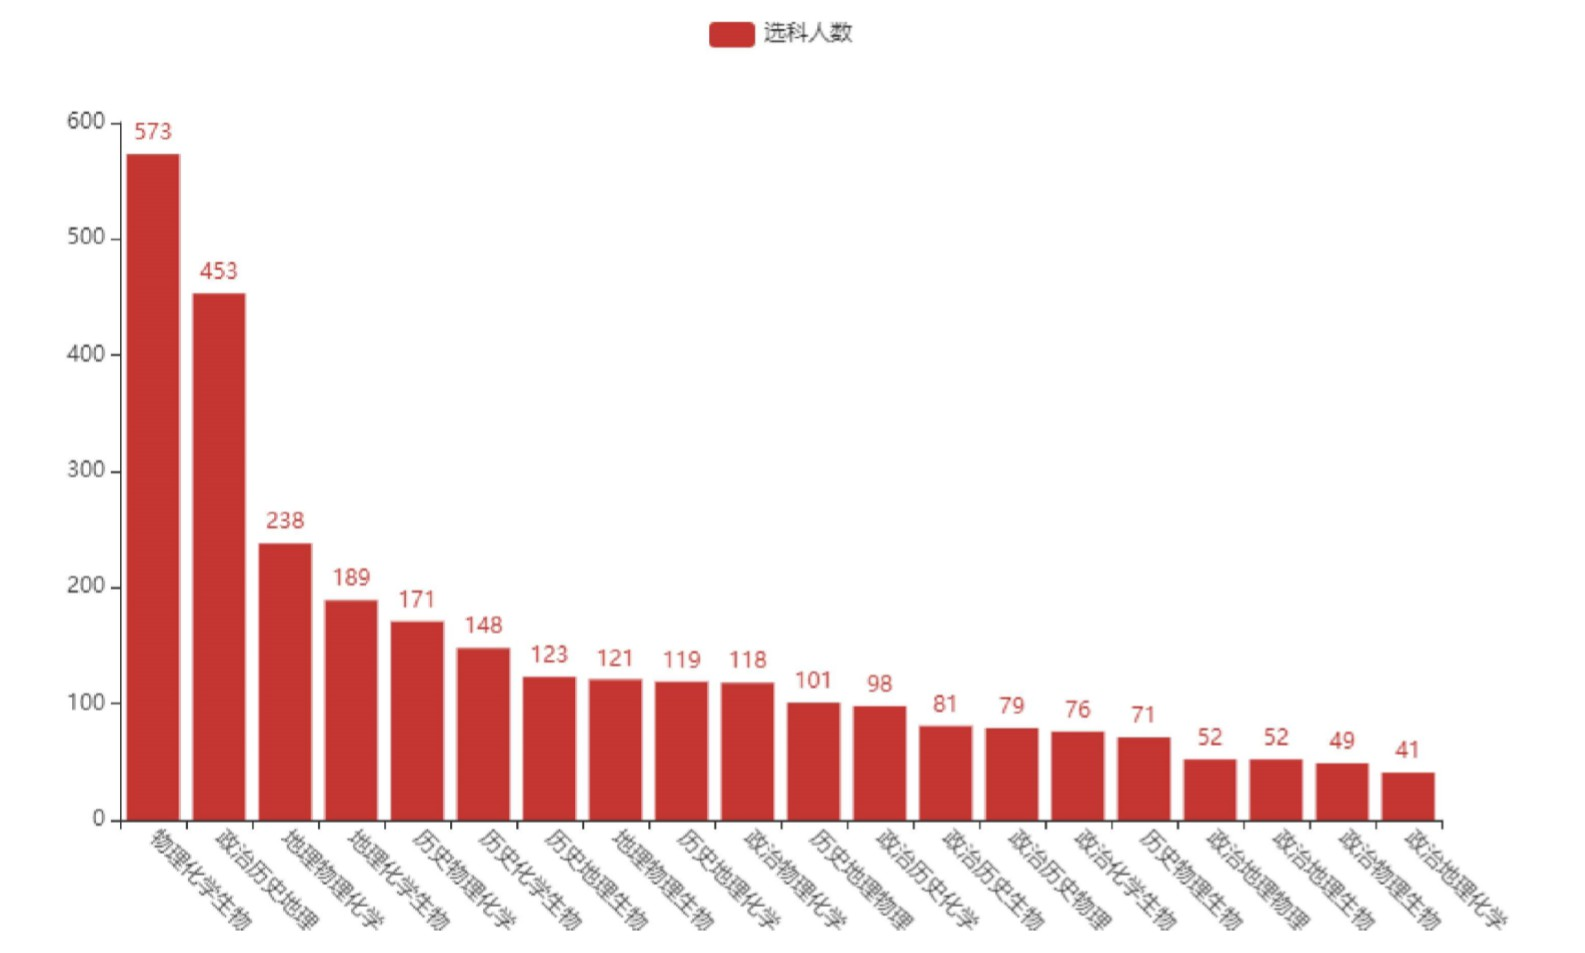
\includegraphics[width=\textwidth]{tab9.jpg}
	\caption{各选课组合实际选择人数}
\end{figure}
\begin{figure}[!ht]
	\centering
	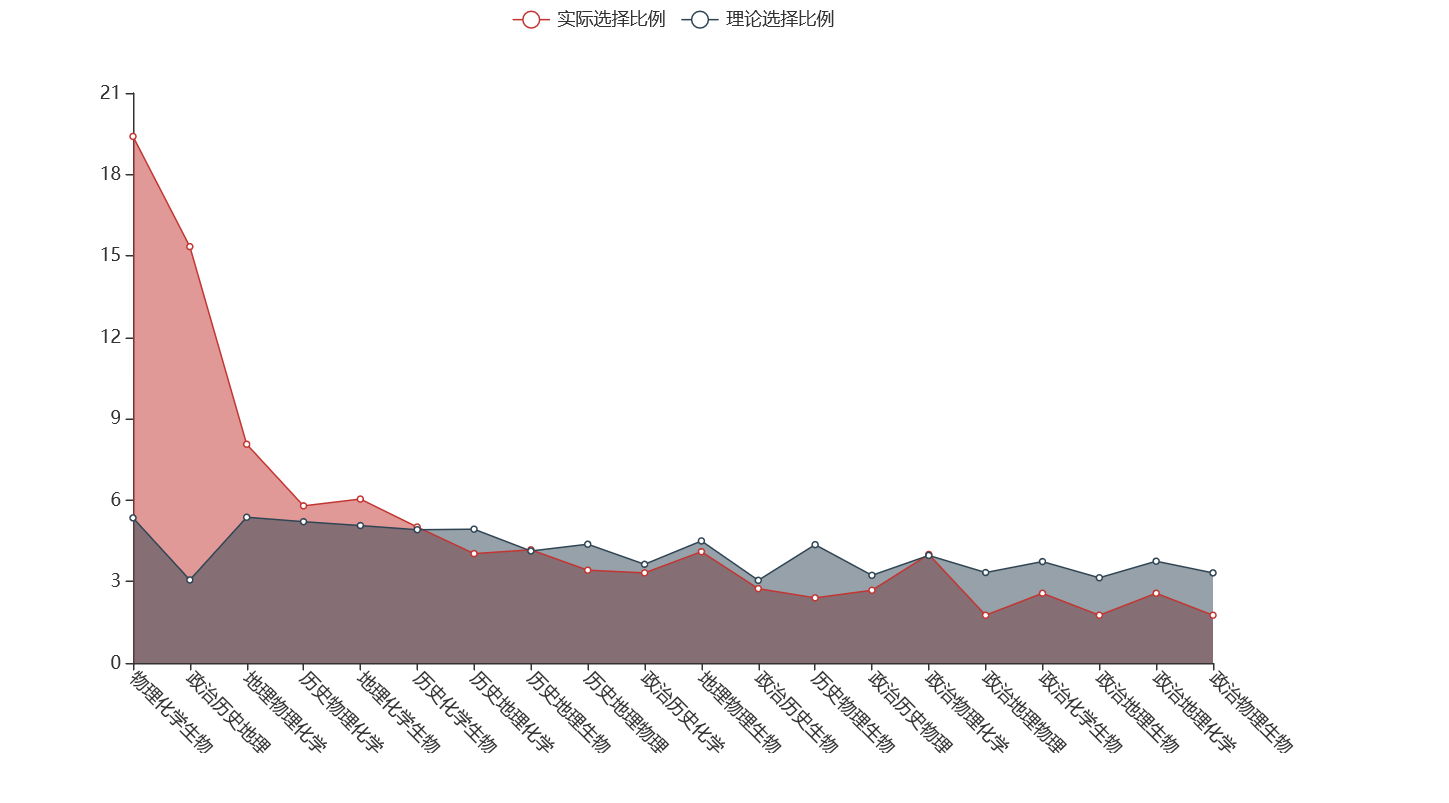
\includegraphics[width=\textwidth]{tab8.png}
	\caption{实际选课数据与理论选科数据对比值}
\end{figure}
\newpage
以物理化学生物为例, 物理17.75\%*化学19.99\%*生物16.74\%=5.35\% ,而实际选科人数达到19.40\%,远高于该比例,猜测擅长物理的人,同时擅长化学与生物的概率较大。而如政治、物理、化学的组合,其实际选择比例大大小于理论值,猜测该三门学科联系较弱,组合选择人数较少。

因此,团队引入学科绑定值,用以衡量学科间联系的紧密性。绑定值计算公式如下。

\begin{equation}
b = \frac{T}{t}
\end{equation}

修正模型误差。修正公式如下。

\begin{equation}
\label{rapired}
T = b*C
\end{equation}

\subsubsection{5.1.6 模型测试}
团队收集到该校另一年级数据,用以代入模型进行测试。测试数据如下表\ref{tab:test}。
% Table generated by Excel2LaTeX from sheet '测试'
	\begin{longtable}{p{2cm}p{4cm}p{4cm}p{3.5cm}}
		
		\caption{\label{tab:test}该高中另一年级选科测试数据}\\
		\toprule
		学科    & \multicolumn{1}{l}{Score(subject)} & \multicolumn{1}{l}{Major(subject)} & \multicolumn{1}{l}{Gender(subject)} \\
		\midrule
		物理    & 7.56787789 & 2.65667 & 0.495195195 \\
		化学    & 7.345757 & -1.74454 & 0.505448997 \\
		生物    & 13.453261 & -2.60533 & 0.503948754 \\
		政治    & 12.78942 & -2.08888 & 0.505046713 \\
		历史    & 13.56345 & -3    & 0.502360237 \\
		地理    & 10.356567 & -8.29995 & 0.500857588 \\
		\bottomrule
	\end{longtable}%

其中,学校教学水平指导值来自该年级某次八校联考成绩;专业选择指导值与表\ref{tab:final_major_value}数值相同;性别指导值中性别选科概率与表\ref{tab:sex_influence}数值相等。该年级共有3256人,其中男生1562人,女生1694人,根据公式\ref{gender}计算得到性别指导值。

将数据导入MEP算法\cite{oltean2002multi},为避免算法不稳定性造成的误差,经过参数调整多次运算,计算其均值作为预测结果,具体测试结果如下表\ref{tab:test_result}所示。

% Table generated by Excel2LaTeX from sheet '测试'
	\begin{longtable}{p{3cm}p{3cm}}
		\caption{\label{tab:test_result}模型初步预测结果}\\
		\toprule
		学科    & \multicolumn{1}{l}{测试结果} \\
		\midrule
		物理    & 0.543599 \\
		化学    & 0.5731226 \\
		生物    & 0.502799 \\
		政治    & 0.3797264 \\
		历史    & 0.465306 \\
		地理    & 0.505447 \\
		\bottomrule
	\end{longtable}%

测试结果为选科人数比值,由于训练集中数值经过标准化处理,故测试结果数值亦向标准化方向靠拢。

由公式\ref{rapired}可得各学科组合预计选科人数及选科结果。预测选课结果如下表\ref{tab:pre_result}所示。

% Table generated by Excel2LaTeX from sheet '20选科预测'

	\begin{longtable}{cccrrrr}
		\caption{\label{tab:pre_result}修正后选科预测结果}\\
		\toprule
		\multicolumn{3}{c}{学科组合} & \multicolumn{1}{l}{预计理论选科比例} & \multicolumn{1}{l}{学科组合绑定值} & \multicolumn{1}{l}{预计选择比例} & \multicolumn{1}{l}{预计选择人数} \\
		\midrule
		\multicolumn{1}{l}{物理} & \multicolumn{1}{l}{化学} & \multicolumn{1}{l}{生物} & 15.66\% & 1.21  & 18.95\% & 616.88  \\
		\multicolumn{1}{l}{政治} & \multicolumn{1}{l}{历史} & \multicolumn{1}{l}{地理} & 8.93\% & 1.67  & 14.93\% & 486.11  \\
		\multicolumn{1}{l}{地理} & \multicolumn{1}{l}{物理} & \multicolumn{1}{l}{化学} & 15.75\% & 0.50  & 7.88\% & 256.54  \\
		\multicolumn{1}{l}{地理} & \multicolumn{1}{l}{化学} & \multicolumn{1}{l}{生物} & 14.57\% & 0.42  & 6.14\% & 199.86  \\
		\multicolumn{1}{l}{历史} & \multicolumn{1}{l}{物理} & \multicolumn{1}{l}{化学} & 14.50\% & 0.37  & 5.37\% & 174.97  \\
		\multicolumn{1}{l}{历史} & \multicolumn{1}{l}{化学} & \multicolumn{1}{l}{生物} & 13.41\% & 0.34  & 4.56\% & 148.57  \\
		\multicolumn{1}{l}{地理} & \multicolumn{1}{l}{物理} & \multicolumn{1}{l}{生物} & 13.81\% & 0.30  & 4.20\% & 136.64  \\
		\multicolumn{1}{l}{历史} & \multicolumn{1}{l}{地理} & \multicolumn{1}{l}{生物} & 11.83\% & 0.34  & 3.98\% & 129.52  \\
		\multicolumn{1}{l}{政治} & \multicolumn{1}{l}{物理} & \multicolumn{1}{l}{化学} & 11.83\% & 0.34  & 3.98\% & 129.46  \\
		\multicolumn{1}{l}{历史} & \multicolumn{1}{l}{地理} & \multicolumn{1}{l}{化学} & 13.48\% & 0.27  & 3.67\% & 119.60  \\
		\multicolumn{1}{l}{历史} & \multicolumn{1}{l}{地理} & \multicolumn{1}{l}{物理} & 12.78\% & 0.26  & 3.33\% & 108.40  \\
		\multicolumn{1}{l}{政治} & \multicolumn{1}{l}{历史} & \multicolumn{1}{l}{化学} & 10.13\% & 0.30  & 3.08\% & 100.26  \\
		\multicolumn{1}{l}{政治} & \multicolumn{1}{l}{历史} & \multicolumn{1}{l}{生物} & 8.88\% & 0.30  & 2.67\% & 86.81  \\
		\multicolumn{1}{l}{政治} & \multicolumn{1}{l}{历史} & \multicolumn{1}{l}{物理} & 9.60\% & 0.28  & 2.65\% & 86.30  \\
		\multicolumn{1}{l}{政治} & \multicolumn{1}{l}{化学} & \multicolumn{1}{l}{生物} & 10.94\% & 0.23  & 2.51\% & 81.81  \\
		\multicolumn{1}{l}{历史} & \multicolumn{1}{l}{物理} & \multicolumn{1}{l}{生物} & 12.72\% & 0.18  & 2.34\% & 76.11  \\
		\multicolumn{1}{l}{政治} & \multicolumn{1}{l}{地理} & \multicolumn{1}{l}{物理} & 10.43\% & 0.18  & 1.84\% & 59.84  \\
		\multicolumn{1}{l}{政治} & \multicolumn{1}{l}{地理} & \multicolumn{1}{l}{生物} & 9.65\% & 0.19  & 1.80\% & 58.71  \\
		\multicolumn{1}{l}{政治} & \multicolumn{1}{l}{物理} & \multicolumn{1}{l}{生物} & 10.38\% & 0.17  & 1.73\% & 56.32  \\
		\multicolumn{1}{l}{政治} & \multicolumn{1}{l}{地理} & \multicolumn{1}{l}{化学} & 11.00\% & 0.12  & 1.36\% & 44.19  \\
		\midrule
		\multicolumn{3}{c}{总} &       &       & 1     & 3256 \\
		\bottomrule
		
	\end{longtable}%

\begin{figure}[!ht]
	\centering
	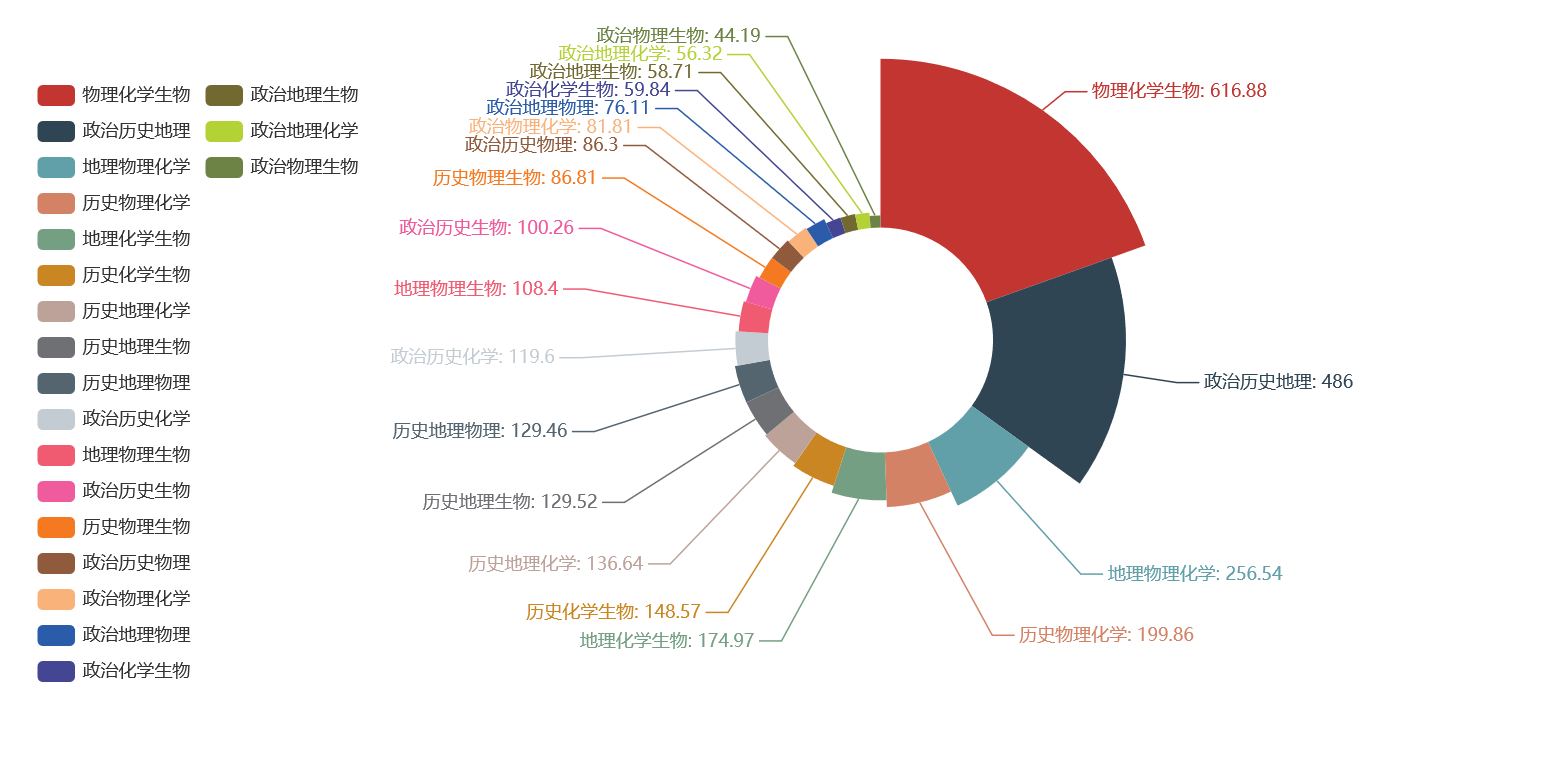
\includegraphics[width=\textwidth]{tab12.png}
	\caption{选科预测结果}
\end{figure}
\newpage

\subsection{问题二及问题三}

面临分科考验的学校,其资源缺口往往来自分科前后资源需求断层。因此寻找资源缺口需比较分科前与分科后资源差距。

\subsubsection{5.2.1 分科前后教师资源情况}
团队收集到2016年山东省部分高中各学科教师数量,即分科政策执行的前一年,各高中各学科教师数量仍保持相对稳定,具体数据如表\ref{tab:teacher_num}。

\begin{longtable}{ccccccc}
	\caption{\label{tab:teacher_num}山东省济南部分重点中学学各学科教师数量}\\
	\toprule
	& 济南一中  & 济南三中  & 山东省实验中学 & 济南中学  & 平均    & 平均占比 \\
	\midrule
	物理    & 19    & 10    & 60    & 20    & 27.25 & 20.49\% \\
	化学    & 19    & 20    & 61    & 18    & 29.5  & 22.18\% \\
	生物    & 13    & 18    & 47    & 17    & 23.75 & 17.86\% \\
	政治    & 8     & 18    & 32    & 15    & 18.25 & 13.72\% \\
	历史    & 12    & 6     & 31    & 15    & 16    & 12.03\% \\
	地理    & 11    & 16    & 32    & 14    & 18.25 & 13.72\% \\
	\bottomrule
\end{longtable}%

团队从山东省教育局官方网站搜集到山东省教师人数及教师平均工资,如下表\ref{tab:teacher_income}所示。
\newpage
% Table generated by Excel2LaTeX from sheet '教师工资'
\begin{longtable}{p{3cm}p{4cm}p{3cm}}
	\caption{\label{tab:teacher_income}山东省教师数量及平均工资}\\
	\toprule
	\multicolumn{1}{l}{年份} & \multicolumn{1}{l}{教师人数 (万人)} & \multicolumn{1}{l}{人均工资} \\
	\midrule
	2013  & 11.9  & 51658 \\
	2014  & 12.16 & 58138 \\
	2015  & 12.52 & 73073 \\
	2016  & 12.96 & 81165 \\
	2017  & 13.44 & 87647 \\
	\bottomrule
\end{longtable}%


假设分科后,各学科对教师教学质量需求均衡,即各科教师平均周课时相等。团队搜集到济南市全市各选科数据,得到各学科各教师人数需求占比如下表\ref{tab:after_teacher_need}。

% Table generated by Excel2LaTeX from sheet '教师工资'
\begin{longtable}{cccc}
	\caption{\label{tab:after_teacher_need}山东省教师数量及平均工资}\\
	\toprule
	学科    & 选科人数  & 选科人数比例 & 教师需求占比 \\
	\midrule
	物理    & 1792  & 11.07\% & 11.07\% \\
	化学    & 2887  & 17.84\% & 17.84\% \\
	生物    & 3382  & 20.90\% & 20.90\% \\
	政治    & 2548  & 15.74\% & 15.74\% \\
	历史    & 2407  & 14.87\% & 14.87\% \\
	地理    & 3169  & 19.58\% & 19.58\% \\
	\midrule
	总     & 16185 & 100.00\% & 100.00\% \\
	\bottomrule
\end{longtable}%


假设表\ref{tab:teacher_num}中四所中学各学科教师平均占比近似于相等于济南市各科教师占比数据,通过计算分科前后需求教师占比与实际教师占比差值,即可得到教师数量缺口数据。即下表\ref{tab:distance_need}所示。

% Table generated by Excel2LaTeX from sheet '教师工资'
\begin{longtable}{ccccc}
	\caption{\label{tab:distance_need}济南市分科后教师数量需求及教师工资资金需求}\\
	\toprule
	学科    & \multicolumn{1}{c}{分科前教师实际占比} & 分科后教师需求占比 & \multicolumn{1}{c}{教师工资资金缺口} & \multicolumn{1}{c}{修正后资金缺口} \\
	\midrule
	物理    & \multicolumn{1}{c}{20.49\%} & 11.07\% & -110926.93  & 0 \\
	化学    & \multicolumn{1}{c}{22.18\%} & 17.84\% & -51158.86  & 0 \\
	生物    & \multicolumn{1}{c}{17.86\%} & 20.90\% & 35795.72  & 35795.72  \\
	政治    & \multicolumn{1}{c}{13.72\%} & 15.74\% & 23808.86  & 23808.86  \\
	历史    & \multicolumn{1}{c}{12.03\%} & 14.87\% & 33474.77  & 33474.77  \\
	地理    & \multicolumn{1}{c}{13.72\%} & 19.58\% & 69006.44  & 69006.44  \\
	\midrule
	总     & 100.00\% & 100.00\% & 0.00  & 162085.79  \\
	\bottomrule
	
\end{longtable}%

其中,由于选科导致的教师需求降低无法在短时间内消失,即教师在选科后较长一段时间内可能存在赋闲情况,因此,将负需求值修正调整为0。结合表\ref{tab:teacher_income}可得到修正后教师工资资金缺口(万元)

\subsubsection{5.2.2 分科前后教室需求情况}

根据山东省政策规定,为保证教学质量,各行政班人数不得超过50人。为方便计算,团队以每班50人为基准。实际生活中,若最后一班人数不足,通常学校会考虑将整个年级同学平均分配,因此,教室数量应向上取整,计算分科前后教室需求情况。

分科前教室数量计算公式如下。
\begin{equation}
\label{equ:before_room}
\Omega_1 = Ceil(\frac{N_1}{50})+Ceil(\frac{N_2}{50})
\end{equation}

分科后,教室需求数量计算公式如下。
\begin{equation}
\label{equ:after_room}
\Omega_2 = \sum\limits_{i=1}^{20}Ceil(\frac{N_0}{50})
\end{equation}

分科前后教室数量差值计算公式如下。
\begin{align}
\label{equ:distance_room}
\varepsilon &= \Omega_2-\Omega_1\\
&=\sum\limits_{i=1}^{20}Ceil(\frac{N_0}{50})- Ceil(\frac{N_1}{50})-Ceil(\frac{N_2}{50})
\end{align}

以曲师大附中为例,由表格\ref{tab:pre_result}预测结果,结合上述公式(\ref{equ:before_room})(\ref{equ:after_room}),计算结果见下表\ref{tab:brfore_room}及表\ref{tab:after_room}。

\begin{longtable}{cccccc}
	\caption{\label{tab:brfore_room}选科后教室需求统计}\\
	\toprule
	\multicolumn{3}{c}{学科组合} & 预计选择人数 & 所需教室  & 所需教室修正值 \\
	\midrule
	\multicolumn{3}{c}{文史类} & 2327  & 46.54  & 47 \\
	\multicolumn{3}{c}{理工类} & 929   & 18.58  & 19 \\
	\midrule
	\multicolumn{3}{c}{总} & 3256  &       & 66 \\
	\bottomrule
	
\end{longtable}%

\begin{longtable}{cccccc}
	\caption{\label{tab:after_room}选科后教室需求统计}\\
	\toprule
	\multicolumn{3}{c}{学科组合} & 预计选择人数 & 所需教室  & 所需教室修正值 \\
	\midrule
	物理    & 化学    & 生物    & 616.88  & 12.34  & 13 \\
	政治    & 历史    & 地理    & 486.11  & 9.72  & 10 \\
	地理    & 物理    & 化学    & 256.54  & 5.13  & 6 \\
	地理    & 化学    & 生物    & 199.86  & 4.00  & 4 \\
	历史    & 物理    & 化学    & 174.97  & 3.50  & 4 \\
	历史    & 化学    & 生物    & 148.57  & 2.97  & 3 \\
	地理    & 物理    & 生物    & 136.64  & 2.73  & 3 \\
	历史    & 地理    & 生物    & 129.52  & 2.59  & 3 \\
	政治    & 物理    & 化学    & 129.46  & 2.59  & 3 \\
	历史    & 地理    & 化学    & 119.60  & 2.39  & 3 \\
	历史    & 地理    & 物理    & 108.40  & 2.17  & 3 \\
	政治    & 历史    & 化学    & 100.26  & 2.01  & 3 \\
	政治    & 历史    & 生物    & 86.81  & 1.74  & 2 \\
	政治    & 历史    & 物理    & 86.30  & 1.73  & 2 \\
	政治    & 化学    & 生物    & 81.81  & 1.64  & 2 \\
	历史    & 物理    & 生物    & 76.11  & 1.52  & 2 \\
	政治    & 地理    & 物理    & 59.84  & 1.20  & 2 \\
	政治    & 地理    & 生物    & 58.71  & 1.17  & 2 \\
	政治    & 物理    & 生物    & 56.32  & 1.13  & 2 \\
	政治    & 地理    & 化学    & 44.19  & 0.88  & 1 \\
	\midrule
	\multicolumn{3}{c}{总} & 3256  &       & 73 \\
	\bottomrule
\end{longtable}%

由公式(\ref{equ:distance_room})知,此次分班后,该校对教室需求数量由66间增长至73间,分班后需求教室增长7间。

\subsubsection{5.2.3 综合分析}
由上述5.2.1师资情况变化,及5.2.2教室数量变化,综合分析可得到分班前后教学资源缺口及其解决条件与可能性。

一个学校的教室数量通常为固定值,无法在短时间内得到补充,因此假设不考虑硬性教室数量,即假设教学楼仍有空余教室或可挪用用于教学的空间,故教学硬件设备方面,可借助教室平均设备造假及教室增长数量,计算教学设备资源缺口及满足条件。其计算公式如下:
\begin{equation}
E = e*\sum\limits_{i=1}^{6}I_i
\end{equation}
其中$I_i$为各科缺口教师数量,$i$从1到6依次为物理、化学、生物、政治、历史、地理科目,若某科教师人数充足,则该科缺口人数自动修正为0。
\begin{align}
Q&=\varepsilon*a+E \\ 
&= \varepsilon*a+e*\sum\limits_{i=1}^{6}I_i
\end{align}

%再整一个表,包含教室增长数量,班主任增长数量,教室教学设备资金需求,等等

\subsection{问题四}
由表\ref{tab:pre_result}知,各选科组合人数从高到低排列如下图\ref{fig:preResult}所示。

\begin{figure}[!ht]
	\centering

	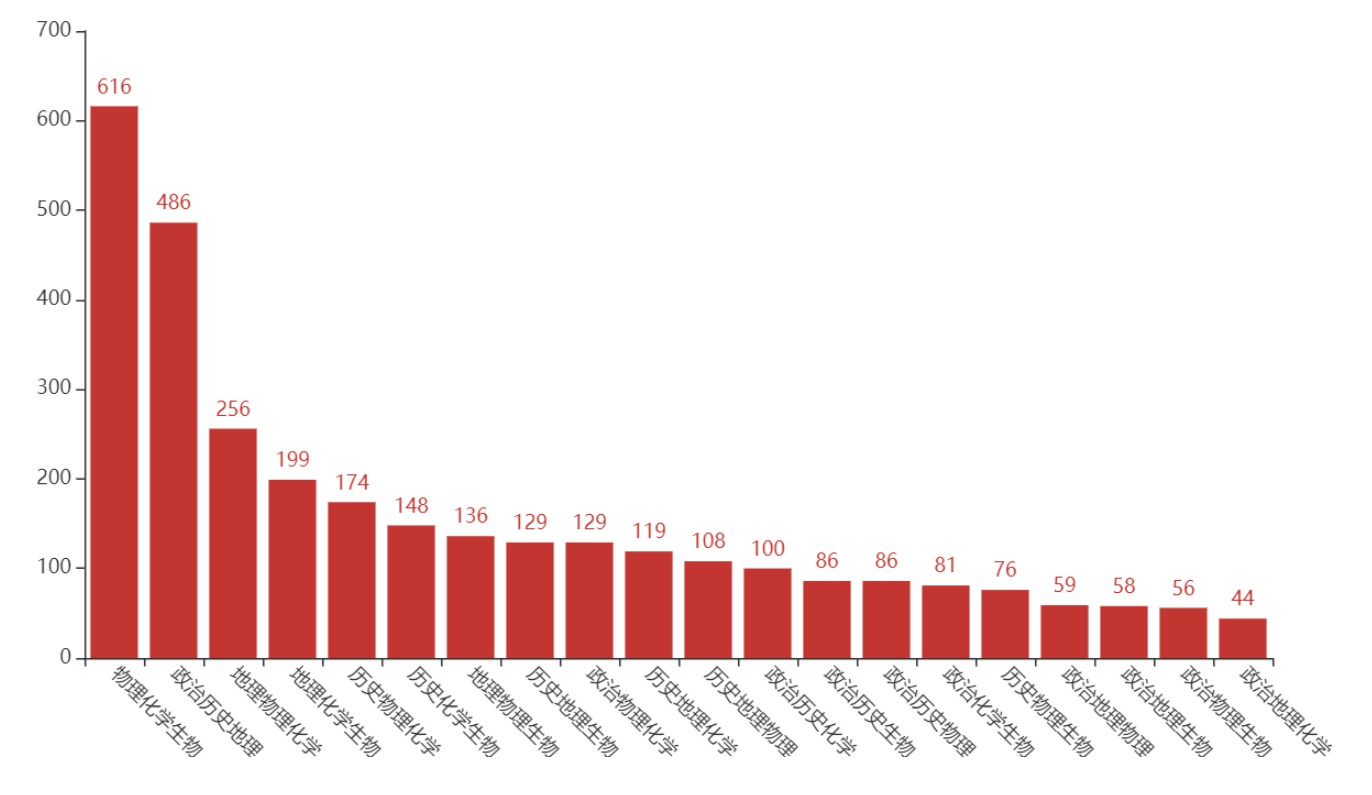
\includegraphics[width=\textwidth]{tab12(4).jpg}
	\caption{各选科组合预测人数}
	\label{fig:preResult}
\end{figure}

由题意,若教育资源有限,应采用“菜单式”选科的方式。而此方案应主要考虑三大问题:选科需求冲突、师资匹配矛盾与教学场地紧缺。为尽可能多地照顾到同学选科需求,应考虑将选科人数多的选科组合进行保留,同时考虑到老师“赋闲”情况的产生,应考虑将选科人数少的单科更多地纳入“菜单”中,避免老师“赋闲”。

可以根据问题一所计算出的各学科间的绑定值,进行学科预组合,并参照问题一估算出的每一种选课组合的选择人数排序结果,取前N(N<20)种组合方式,列入“菜单”的选科“套餐”中,以提供学生进行选科参考并方便排课。此外,针对另外(20-N)种冷门学科组合的情况,建议可以尝试“学校联盟”的方式解决。

由于各学校的优势学科、生源质量、教师分配各不相同,因此导致各学校的选科组合情况也各有差异,如新高考改革前相对偏理科的学校,可能政治、历史和地理的教学资源就较为短缺,因此可以考虑在地理位置上相对集中的某几所学校采用区域性跨学校式走班的模式。这样既解决了所有同学的选科需求,又能充分发挥各学校的优势学科教学资源。

为尽可能达到教师资源高水平匹配的目标,要合理设置“选课走班”的教学类型和班级规模。相信每所学校在新高考改革后的选科问题上更多出现的情况为,热门学科教师资源紧缺,除了可以人为操控学科教学班级的规模,还可以在教学类型上有所创新,如可尝试利用互联网与实时视频传输技术,进行课程直播或线上答疑等。同时也考虑到老师“赋闲”情况的产生,应选择性地将选科人数少的单科更多地纳入“菜单”中,使各学科教师各有所职。

为尽可能合理安排各学科教学场地,可以采用不同程度的走班制度,大致可以分为“不走班”、“微走班”、“全走班”。“不走班”,是指学校向学生提供有限数量的选科组合,然后将三门选考科目均相同的学生组成一个班,学生在固定的教室上课,类似于改革前的文理分班情况。“微走班”,是指部分学生或科目走班,即将一门或两门选科相同的学生优先组成行政班级,其他科目或学生走班教学。“全走班”,针对的是问题一的选科组合人数排序中位于最后几列的情况,此类学生较少,所有学生所有科目均通过走班完成教学。

无论采用哪种方案,都需要学校在尊重学生意愿与自身资源条件限制之间找到合适的平衡点,从而做出最为合理的选择,以此达到教师的数量、结构与学生选课走班之间的最大平衡。


\subsection{问题五}
排课问题是学校制定教学计划、安排教学过程中的一项较为复杂的工作,在学校教务管理工作中处于重要地位。学校在每学期末都要根据培养计划和教学资源作出下学期的教学安排,这主要体现在对课表的编排上。其中涉及的关键要素很多,包括教师、班级、教室和授课时段等。根据排课总体目标、约束条件及优先级,充分利用紧缺资源,设计并实现课表的安排。

排课时应避免各种冲突,包括但不限于:
\begin{enumerate}
	\item 教室不冲突,同一教室同一时间不能安排两门课程,人数不能超过教室的最大容量;
	\item 学生不冲突,同一班级学生不能在同一时间
	上两门或两门以上课程;
	\item 课程不冲突,同一班级同一课程不能同一时间在不同地点上课;
	\item 教师不冲突,同一教师不能同一时间在不同地点上课。
\end{enumerate}

排课问题建模的复杂处之一,就是在于问题抽象的难度。如何将教室、教师、学生、时间等诸多复杂且相互排斥的因素抽象为人脑及机器可理解的语言、变量或符号,成为当前排课问题研究的热点之一。


\subsubsection{算法选择}
该问题可归类为多约束优化问题,团队拟采用遗传算法(Genetic  Algorithms,GA)\cite{gen2007genetic}尝试解决此问题\cite{顾运筠2006遗传算法应用于排课问题中的教师安排最优化}\cite{唐勇2002基于遗传算法的排课系统}。在解决的过程中,发现遗传算子在染色体交叉过程中存在交叉互斥问题。

考虑到排课问题与0-1背包问题在某些程度上拥有较高相似性,因此,在交叉环节,拟采用禁忌搜索算法对其进行约束\cite{mantawy1999integrating}\cite{李大卫1998遗传算法与禁忌搜索算法的混合策略},以保证交叉后的算子仍保持可行状态,减少后续工作量。

由于禁忌搜索算法天然的严格性,导致算法在运算过程中,占用大量的资源进行边界条件的判定及变量比较,且如何设置禁忌表、禁忌期限与渴望准则,亦成为难点之一。因此,团队考虑在遗传算法交叉环节中,只保留禁忌搜索算法经典的回溯思想,将其余不重要的因素抛弃;在变异环节,考虑将一周时间内各班级课程随机互换,以达到变异效果。

\subsubsection{数学建模}
根据上述问题描述,排课问题中涉及到教学班、课程、教师、教室和时间等相互制约的因素,其制约因素数学表达如下表\ref{tab:Algorithms_char}所示。
\begin{longtable}{cc}
	\caption{\label{tab:Algorithms_char}遗传算法符号}\\
	\toprule
	字段名   & 数学表达 \\
	\midrule
	学生集   & S=\{s1,s2,s3,…,sn\} \\
	课程集   & C=\{c1,c2,c3,…,cn\} \\
	任课教师集 & T=\{t1,t2,t3…,tn\} \\
	时间段集  & P=\{p1,p2,p3,…,pn\} \\
	教室集   & R=\{r1,r2,r3,…,rn\} \\
	\bottomrule	
\end{longtable}%
“走班制”模式的排课过程没有“行政班”的概念,基于学生选课情况对学生按选课情况进行分组形成不同的教学班,其中教学班、教师和课程作为一个授课安排,教室、时间段作为一个教室时间安排,因此排课问题可以演化成为任意授课安排寻找满足约束条件的教室时间对问题.

软约束条件为在实际的排课过程中,根据不同的排课对象的特殊性制定的优化条件,在解决排课问题时是否遵守了软约束条件将会给排课结果带来很大的影响,排课算法多大程度符合软约束规则,便会得到相应程度优质的解.具体如下:
\begin{enumerate}
\item 一门课程的多次上课时间段的分配尽量均匀.
\item 一个学生的所有课程分布不应过度集中,避免某段时间过于空闲.
\item 上课教室的座位数和上课的教学班的人数相差适中,保证教室的利用率.
\item 同一个教师的相近时间段的教学尽量安排在相对固定的教室或相近教室.
\item 艺体课程应避免安排在早上和下午的一、二节次。
\item 逻辑性强的课程尽量安排在教学效果好的
上课节次,
\item 公共课及学时多的课应优先安排.
\item 每个教学班的人数不宜过少也不宜过多.
\item 对于上课时间确定的教师,首先确保满足其上课时间.
\item 对学生分组的组数要尽量小于需要进行教学分层的课程数量,将软、硬约束写入课程的基因中,减少遗传操作中无效课表产生的比例,提高有效课表的合理性.
\end{enumerate}

\subsubsection{基因编码}
自然界里的物种遗传由染色体决定,不同的染色体决定不同物种之间存在的差异,而每种物种特有的遗传信息存放在染色体内,遗传信息按一定的模式排列,即进行了遗传编码。

以实施了“走班制”教学模式的某高中学校为例,设计了一组适合该校特定情况的基因编码方式。排课得到的课表作为一条染色体,课表中的信息(排课记录)作为染色体上不同的基因。以总教学时间段数为行数,以已经被分配教师和课程的教学班数(各组教学班总数)为列数,组成二维表,在表内非空单元放入教室编号,涉及的排课信息采用二进制编码方式表示,染色体编码方案如图\ref{fig:RST_pic}所示。
\begin{figure}[!ht]
	\centering

	
\includegraphics[width=\textwidth]{GA-stru.png}
	\caption{染色体编码方案}	
	\label{fig:RST_pic}
\end{figure}
\subsubsection{设计适应度函数}

排课问题作为多组合目标规划问题,受到多个约束条件的影响,如:各个课程在教学时间段分配的均匀度、学生课程安排均匀度、教室资源利用率以及课程时间段安排优度等,将这些约束条件的综合评价作为算法的适应度函数。

\subsubsection{选择算子}
排课算法中,选择操作是基于适应度进行优胜略汰的过程。算法根据种群中每个个体的适应度大小,保留第g代中优越的候选解进入第g+1代,放弃其他一些非优的候选解。其中个体适应度越大,个体基因的优值越高,被遗传到下一代种群的概率就越高,为了避免在此过程中出现的种群早熟早收敛现象,算法在选择操作时引入了竞争机制的同时采用了是轮盘赌算法。

具体操作为,找到g代种群中最大奖励值和最大适应度值,调用轮盘赌算法方法,首先以轮盘安置方式按种群适应度降序排列,设置随机值r,采用二分查找的方式查找r在轮盘中对应位置设为d,该位置为要选择的染色体位置。

\subsubsection{交叉算子}
在交叉操作过程中,通过将第g代种群中所有个体随机的进行两两配对,产生更高效、合理的新个体解。为解决传统遗传算法在交叉操作时用来作为搜索解的空间相对较小的问题,采用计算编码间的海明距离的方式,使得每两对个体都有部分染色体相互交换,产生新个体,保持群体的多样性,从而提高了种群变化的效率,避免早熟现象。针对每个个体进行交叉操作预测,产生随机值rd,根据选择操作中计算的种群最大适应度、参数、该染色体的适应度计算交叉概率,若rd小于交叉概率则进行交叉操作,并通过轮盘赌法找到与当前染色体进行交叉操作的位置,实现交叉操作。

\subsubsection{变异算子}
变异操作作为算法产生新个体的辅助方法,将个体染色体的部分基因编码随机交换,达到产生新个体的目的。为了扩大了遗传算法中搜索区域的范围,同时提高了种群变化的效率以及种群最优解搜索能力,变异概率的设置与交叉概率类似,采用自适应方式。

种群中染色体的基因编码(课程信息)以自适应的概率变异,若变异,则随机一个课程时间段安排与之交换。

\subsubsection{算法运行结果}
算法运行结果如下图\ref{fig:GA_pic}所示。最终排课情况如表\ref{tab:class_result}所示。
\begin{figure}[!ht]
	\centering

	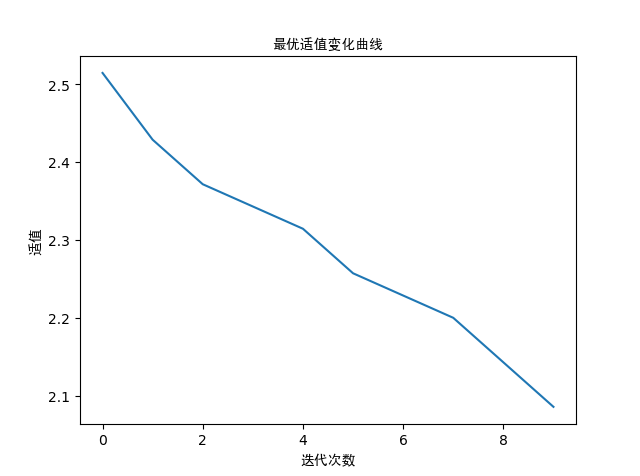
\includegraphics[width=0.8\textwidth]{Figure3.png}
	\caption{算法运行结果}	
	\label{fig:GA_pic}
\end{figure}


\begin{landscape}
	\begin{longtable}{llllllllllllllll}
		\caption{\label{tab:class_result}最终排课情况}\\
		\toprule
		& \multicolumn{5}{c}{一班}                & \multicolumn{5}{c}{二班}                & \multicolumn{5}{c}{三班} \\
		\midrule
		节次    & 星期一   & 星期二   & 星期三   & 星期四   & 星期五   & 星期一   & 星期二   & 星期三   & 星期四   & 星期五   & 星期一   & 星期二   & 星期三   & 星期四   & 星期五 \\
		\midrule
		一     & 历史    & 政治    & 英语    & 语文    & 生物    & 无     & 地理    & 数学    & 地理    & 语文    & 无     & 英语    & 无     & 数学    & 无 \\
		二     & 化学    & 数学    & 物理    & 无     & 历史    & 物理    & 英语    & 无     & 英语    & 化学    & 语文    & 语文    & 历史    & 无     & 语文 \\
		三     & 英语    & 无     & 数学    & 数学    & 英语    & 无     & 历史    & 无     & 英语    & 无     & 生物    & 无     & 无     & 化学    & 地理 \\
		四     & 生物    & 无     & 政治    & 无     & 物理    & 数学    & 政治    & 历史    & 语文    & 无     & 无     & 历史    & 数学    & 无     & 语文 \\
		五     & 语文    & 英语    & 地理    & 无     & 语文    & 物理    & 无     & 英语    & 无     & 语文    & 物理    & 物理    & 无     & 政治    & 政治 \\
		六     & 无     & 无     & 地理    & 语文    & 化学    & 化学    & 政治    & 无     & 生物    & 生物    & 数学    & 生物    & 英语    & 英语    & 地理 \\
		七     & 无     & 数学    & 无     & 无     & 无     & 无     & 语文    & 数学    & 无     & 数学    & 化学    & 无     & 数学    & 英语    & 无 \\
		\midrule
		&       &       &       &       &       &       &       &       &       &       &       &       &       &       &  \\
		\midrule
		& \multicolumn{5}{c}{四班}                & \multicolumn{5}{c}{五班}                & \multicolumn{5}{c}{六班} \\
		\midrule
		节次    & 星期一   & 星期二   & 星期三   & 星期四   & 星期五   & 星期一   & 星期二   & 星期三   & 星期四   & 星期五   & 星期一   & 星期二   & 星期三   & 星期四   & 星期五 \\
		\midrule
		一     & 数学    & 无     & 化学    & 生物    & 物理    & 政治    & 生物    & 无     & 无     & 历史    & 地理    & 化学    & 英语    & 数学    & 政治 \\
		二     & 历史    & 历史    & 地理    & 语文    & 无     & 政治    & 无     & 物理    & 数学    & 英语    & 语文    & 无     & 无     & 英语    & 无 \\
		三     & 无     & 英语    & 无     & 无     & 政治    & 地理    & 无     & 化学    & 英语    & 数学    & 无     & 数学    & 英语    & 无     & 语文 \\
		四     & 生物    & 英语    & 无     & 语文    & 英语    & 语文    & 无     & 数学    & 化学    & 无     & 无     & 生物    & 无     & 物理    & 历史 \\
		五     & 数学    & 化学    & 无     & 地理    & 数学    & 语文    & 语文    & 英语    & 英语    & 语文    & 化学    & 无     & 无     & 物理    & 无 \\
		六     & 无     & 语文    & 数学    & 无     & 无     & 生物    & 无     & 无     & 地理    & 历史    & 语文    & 政治    & 地理    & 数学    & 无 \\
		七     & 语文    & 无     & 政治    & 物理    & 英语    & 无     & 物理    & 无     & 数学    & 无     & 语文    & 生物    & 英语    & 历史    & 数学 \\
		\bottomrule
	\end{longtable}%
\end{landscape}
	



\bibliographystyle{ieeetr}
\bibliography{ref}



\newpage
\appendix
\section{Python排课算法源程序}
\lstset{language=Python}
\begin{lstlisting}
import matplotlib
import pandas
import numpy as np
import random
from  collections import Counter
from matplotlib import pyplot as plt

def random_class():
class_num = 6
class_list = np.zeros((class_num, 5, 7))
for i in range(class_num):  # 一个班
subject_CME = np.zeros(3)
subject_PCBPHG = np.zeros(6)
while (np.sum(subject_CME == 4) < 3 or np.sum(subject_PCBPHG == 2) < 6):
j = int(random.random() * 5)
k = int(random.random() * 7)
subject = int(random.random() * 9 + 1)
if (class_list[i][j][k] == 0):
if (subject <= 3):  # 主科
if (subject_CME[subject - 1] < 4):  # 主科未满
subject_CME[subject - 1] += 1
class_list[i][j][k] = subject
else:  # 副科
if (subject_PCBPHG[subject - 4] < 2):  # 副科未满
subject_PCBPHG[subject - 4] += 1
class_list[i][j][k] = subject
return class_list

def ave_counter():
class_num = 6
class_list = random_class()[:]

fitness_class = np.zeros((7*5,class_num))
class_re = np.zeros((5,7,class_num))
for k in range(7):
for j in range(5):
for i in range(class_num):
class_re[j][k][i] = class_list[i][j][k]
fitness_class[j*7+k] = class_re[j][k]

sum = 0
for i in range(5*7):
sum += Counter(fitness_class[i]).most_common(1)[0][-1]

ave = sum/(5*7)
return ave,class_list


fitness_best,best_course_list = ave_counter()
fitness_per = []
# course_list_per = []
fitness_per.append(fitness_best)
for i in range(1000):
fitness,course_list = ave_counter()
if(fitness<fitness_best):
fitness_best=fitness
best_course_list = course_list
fitness_per.append(fitness_best)

print(fitness_best)
print(best_course_list)
x = np.arange(len(fitness_per))
y = fitness_per

zhfont1 = matplotlib.font_manager.FontProperties(fname="SimHei.ttf") 
plt.title("最优适值变化曲线",fontproperties=zhfont1)
plt.xlabel("迭代次数",fontproperties=zhfont1)
plt.ylabel("适值",fontproperties=zhfont1)
plt.plot(x,y)
plt.show()
\end{lstlisting}


\section{MEP多表达式编程源程序}
\lstset{language=Python}
\begin{lstlisting}
#include <math.h>
#include <stdio.h>

void mepx(double *x /*inputs*/, double *outputs)
{
//constants ...
double constants[5];
constants[0] = 0.770643;
constants[1] = 0.321319;
constants[2] = 0.609742;
constants[3] = 0.786920;
constants[4] = 0.838836;

double prg[100];
prg[0] = x[0];
prg[1] = x[0];
prg[2] = sin(prg[0]);
prg[3] = x[1];
prg[4] = x[2];
prg[5] = cos(prg[1]);
prg[6] = fabs(prg[5]);
prg[7] = pow(prg[0], prg[4]);
prg[8] = x[1];
prg[9] = constants[1];
prg[10] = prg[9] + prg[6];
prg[11] = x[2];
prg[12] = x[2];
prg[13] = prg[2] * prg[7];
prg[14] = x[0];
prg[15] = ceil(prg[8]);
prg[16] = pow(10, prg[13]);
prg[17] = x[1];
prg[18] = x[2];
prg[19] = fabs(prg[11]);
prg[20] = prg[14] / prg[7];
prg[21] = x[0];
prg[22] = x[0];
prg[23] = constants[1];
prg[24] = prg[17] * prg[17];
prg[25] = x[1];
prg[26] = x[2];
prg[27] = x[2];
prg[28] = sin(prg[2]);
prg[29] = fabs(prg[13]);
prg[30] = x[2];
prg[31] = x[0];
prg[32] = x[1];
prg[33] = x[0];
prg[34] = x[0];
prg[35] = x[1];
prg[36] = tan(prg[28]);
prg[37] = constants[1];
prg[38] = prg[21] > prg[18]?prg[21] : prg[18]; // max
prg[39] = tan(prg[5]);
prg[40] = constants[3];
prg[41] = x[0];
prg[42] = sin(prg[36]);
prg[43] = x[0];
prg[44] = x[0];
prg[45] = constants[2];
prg[46] = prg[32] > prg[15]?prg[32] : prg[15]; // max
prg[47] = x[2];
prg[48] = x[1];
prg[49] = x[2];
prg[50] = -prg[23];
prg[51] = x[1];
prg[52] = x[2];
prg[53] = sin(prg[20]);
prg[54] = prg[53] * prg[53];
prg[55] = x[1];
prg[56] = prg[14] - prg[55];
prg[57] = x[1];
prg[58] = prg[9] + prg[46];
prg[59] = prg[51] * prg[53];
prg[60] = x[2];
prg[61] = x[0];
prg[62] = floor(prg[35]);
prg[63] = x[1];
prg[64] = x[2];
prg[65] = x[0];
prg[66] = constants[2];
prg[67] = prg[50] * prg[10];
prg[68] = prg[54] < prg[16]?prg[54] : prg[16]; // min
prg[69] = pow(10, prg[34]);
prg[70] = tan(prg[59]);
prg[71] = x[2];
prg[72] = x[2];
prg[73] = tan(prg[55]);
prg[74] = x[1];
prg[75] = tan(prg[68]);
prg[76] = x[2];
prg[77] = x[2];
prg[78] = x[1];
prg[79] = x[1];
prg[80] = x[0];
prg[81] = x[1];
prg[82] = x[2];
prg[83] = constants[3];
prg[84] = sin(prg[49]);
prg[85] = x[1];
prg[86] = x[0];
prg[87] = constants[0];
prg[88] = x[0];
prg[89] = x[1];
prg[90] = x[1];
prg[91] = cos(prg[23]);
prg[92] = x[0];
prg[93] = x[2];
prg[94] = constants[0];
prg[95] = x[1];
prg[96] = prg[49] - prg[87];
prg[97] = x[1];
prg[98] = x[2];
prg[99] = sin(prg[68]);

outputs[0] = prg[75];
}

int main(void)
{

//example of utilization ...

double x[3];
x[0] = 7.073398;
x[1] = 2.656670;
x[2] = 0.490953;

double outputs[1];

mepx(x, outputs);
printf("%lf", outputs[0]);
getchar();
}

\end{lstlisting}

\end{document} 